%Folgende Zeile aktivieren und als SVN property "svn:keywords" auf "Id" setzen, um SVN Versionsinformationen im Dokument zu erhalten
%\svnInfo $Id: einleitung.tex 60 2012-01-26 15:56:06Z koppor $ 

\chapter{Selektion gut detektierbarer Bilder}
\label{chap:slk}
	Um aus dem beschriebenen Bilderstack möglichst gut detektierbare Einzelbilder zu erhalten, werden hier verschiedene Verfahren vorgestellt, die eine weitgehend automatische Auswahl von Bildern erstellt, die für die weitere Objekterkennung gut geeignet sind. \\
Da der gescannte Mikrochip aus vier Leiterbahnschichten besteht, muss der beim Scannen entstehende Bilderstack in vier Intervalle eingeteilt werden, welches jeweils eine Leiterbahnschicht repräsentiert. 
\begin{figure}[H]
  \begin{center}
    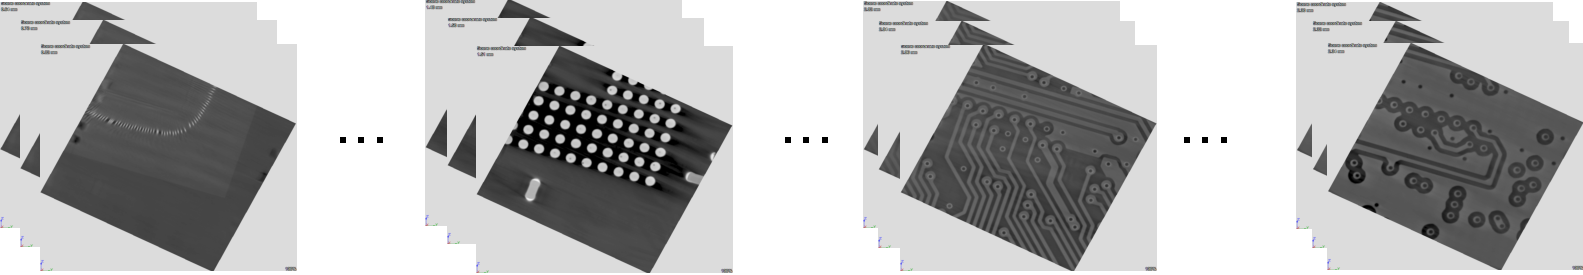
\includegraphics[width=\textwidth]{stack.pdf}
    \caption{Einteilung des Bilderstacks in vier Intervalle}
    \label{fig:intervalls}
  \end{center}
\end{figure}
Ziel der unten vorgestellten Verfahren besteht darin, um für jedes Intervall das Bild zu finden, dass die Leiterbahnschicht am genausten repräsentiert.
Die aus den Verfahren gewonnen Bilder werden anschließend weiterverwendet, d.h. es werden die 2D Objekterkennungsverfahren darauf angewandt und bewertet, wie gut die ausgewählten Bilder für die einzelnen Verfahren geeignet sind, und ob für jedes Intervall tatsächlich das am besten detektierbare Bild gefunden wurde.

\section{Binärbilder}
Bei diesem Verfahren werden zunächst alle Bilder in Binärbilder umgewandelt. Als binärer Schwellwert wird dabei der Wert 70 gewählt, d.h. alle Pixel, deren Grauwert größer als 70 ist, wird der Grauwert 255 zugewiesen, allen Pixeln die einen Grauwert kleiner, bzw. gleich 70 besitzen, wird der Grauwert 0 zugewiesen. Anschließend wird das Bild ausgewählt, welches die maximale Anzahl an weißen Pixeln (Pixel mit dem Grauwert 255) besitzen.

Die Idee, die hinter diesem Verfahren steckt ist, dass Bilder, die eine möglichst große Anzahl von Pixeln mit maximalen Grauwert besitzen, viele Objekte enthalten, die detektiert werden können.

\section{Canny-Edge-Bilder}
Bei diesem Verfahren werden die einzelnen Bilder der Intervalle zunächst mit dem Canny-Edge Operator in die entsprechenden Kantenbilder überführt. Anschließend werden die Kantenpixeln in den Kantenbildern gezählt, wobei für jedes Intervall das Bild ausgewählt wird, dass die meisten Kantenpixel besitzt.\\

Der Ansatz hierbei ist, dass Bilder, die viele einzelne Objekte enthalten, mehr Kantenpixel liefern, als Bilder, in denen wenige Objekte enthalten sind.

\section{Hough-Transformation}

\section{Lokaler Kontrast}
	


